\documentclass[11pt,a4paper]{article}
\usepackage[latin5]{inputenc}
\usepackage[english]{babel}
\usepackage{amsmath}
\usepackage{amsfonts}
\usepackage{amssymb}
\usepackage{graphicx,subfig}
\author{Alexander Attinger, Yannic Kilcher}
\title{Report Blatt 1}

\begin{document}
\maketitle
\section{Excercise 1}
The Histogram of a nice, contranst rich picture is broad and relatively flat, all photographers know that. Images with a narrow histogram such as can be seen in Fig. \ref{fig:eq} a), usually lack contrast. Histogram equalization is an important technique to enhance contrast. It is a technique, where intensities of pixels will be mapped to different values such that the histogram of the transformed image will look flatter. Ideally, a histogram should resemble a uniform distribution after the transformation. This cannot be obtained bc of the intensities can only take discrete values (compare Fig.\ref{fig:eq}d). Nevertheless, histogram equalization improves contrast and image quality markedly, as can be seen in Fig. \ref{fig:eq}b).



\begin{figure}%
\centering
\subfloat[]["Original Image"]{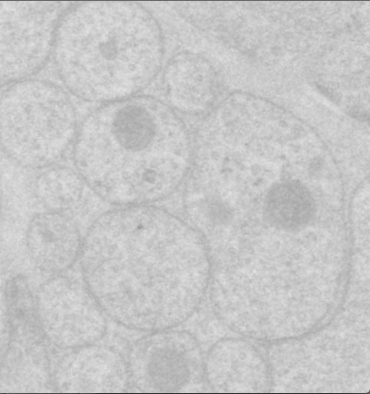
\includegraphics[scale=.4]{pics/neuron_orig.png}}
\quad
\subfloat[]["After hist. equalization"]{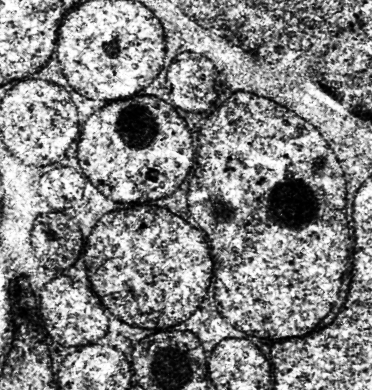
\includegraphics[scale=.4]{pics/neuron_eq.png}}
\quad
\subfloat[]["Histogram of original]{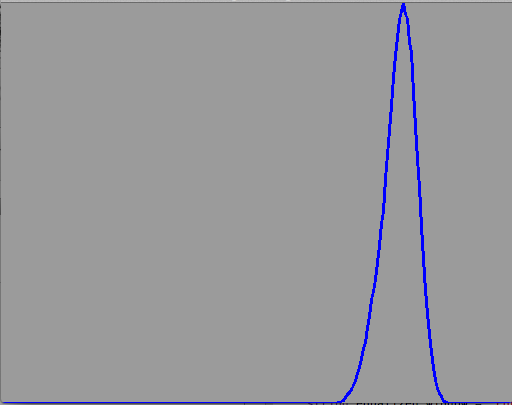
\includegraphics[scale=.3]{pics/hist_orig.png}}
\quad
\subfloat[]["Equalized Histogram"]{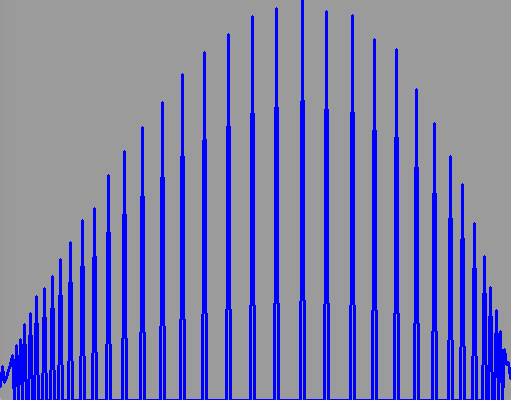
\includegraphics[scale=.3]{pics/hist_eq.png}}
\caption{Histogram Equalization. Image of neurons before and after histogram equalization. The contrast is markedly improved.}%
\label{fig:eq}%
\end{figure}

\section{Exercise 2}
\subsection{Smoothing}

In this exercise we are presented with two images of the same scene. Artificial noise has been added to both images, in image one, it looks like it was white noise, whereas in image 2 it looks more like a salt-and-pepper kind of noise. Smoothing or blurring is a frequently used technique to reduce noise in an image. There are different kind of filters. We were asked to use and compare three: Gaussian Blur, Median Blur and normal Blur.
\paragraph{Blur}
The blur filter or normalized box filter is the most simple linear filter. Each output pixel is just the mean of all $n*n$ pixel surrounding it.
\paragraph{Gaussian Blur}
Another frequently used linear filter. The value of each output pixel is now determined by the weighted mean of its neighbours. The weights are determined by a bivariate gaussian distribution. It is probably one of the most frequently used filters for noise reduction.	
\paragraph{Median Blur}
The median blur is a non linear filter, since the computation of the median is a non-linear operation. The value of an output pixel is determined by the median of its surrounding neigbours.

\subsection{Applying the filters}
The results of applying the normalized box filter can be seen in Fig.\ref{fig:blur}. I used the function \textit{blur} of the OpenCV API to apply blur filters of different kernel size. Only the images for the 3x3 and the 9x9 kernels are shown. Similarly, the application of the gaussian filter can be seen in Fig.\ref{fig:gblur}, and the results of the median filters is shown in Fig. \ref{fig:mblur}.

\begin{figure}%
\centering
\subfloat[]["Original Image 1"]{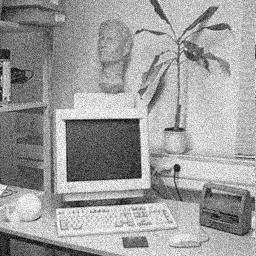
\includegraphics[scale=.5]{pics/office-noisy-1.jpg}}
\quad
\subfloat[]["Image 2"]{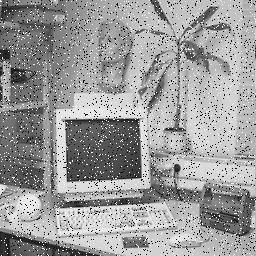
\includegraphics[scale=.5]{pics/office-noisy-2.jpg}}
\quad
\subfloat[]["Blur filter Im 1 5x5"]{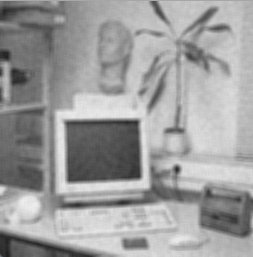
\includegraphics[scale=.5]{pics/1blur_5.png}}
\quad
\subfloat[]["Blur filter Im 2 5x5"]{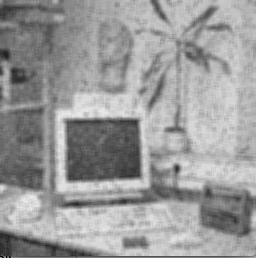
\includegraphics[scale=.5]{pics/2blur_5.png}}
\quad
\subfloat[]["Blur filter Im 1 9x9"]{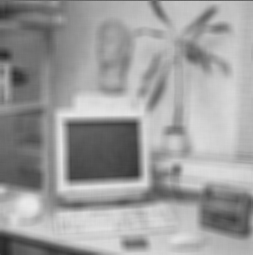
\includegraphics[scale=.5]{pics/1blur_9.png}}
\quad
\subfloat[]["Blur filter Im 2 9x9"]{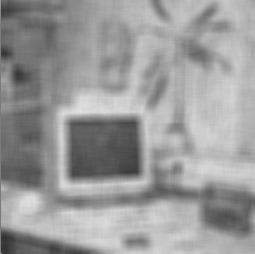
\includegraphics[scale=.5]{pics/2blur_9.png}}
\quad

\caption{Comparison of different filter kernel size for blur filter.}%
\label{fig:blur}%
\end{figure}

\begin{figure}%
\centering
\subfloat[]["Original Image 1"]{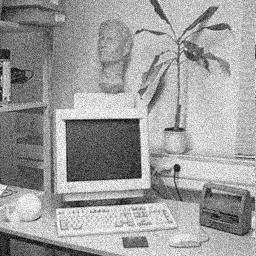
\includegraphics[scale=.5]{pics/office-noisy-1.jpg}}
\quad
\subfloat[]["Image 2"]{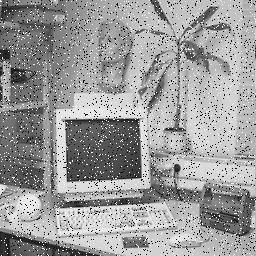
\includegraphics[scale=.5]{pics/office-noisy-2.jpg}}
\quad
\subfloat[]["Gaussian Blur filter Im 1 5x5"]{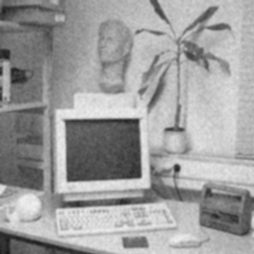
\includegraphics[scale=.5]{pics/1gauss_5.png}}
\quad
\subfloat[]["Gaussian Blur filter Im 2 5x5"]{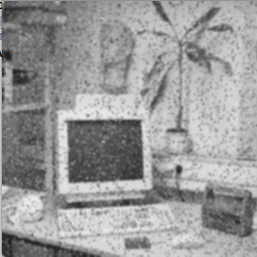
\includegraphics[scale=.5]{pics/2gauss_5.png}}
\quad
\subfloat[]["Gaussian Blur filter Im 1 9x9"]{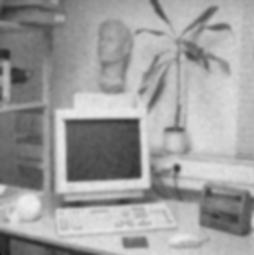
\includegraphics[scale=.5]{pics/1gauss_9.png}}
\quad
\subfloat[]["Gaussian Blur filter Im 2 9x9"]{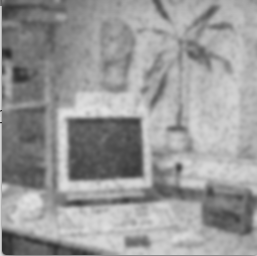
\includegraphics[scale=.5]{pics/2gauss_9.png}}
\quad

\caption{Comparison of different filter kernel size for Gaussian blur filter. The 3x3 kernel works very good in reducing the artificial noise of image 1. However, the filter does not work well for image 2 with a different kind of noise}%
\label{fig:gblur}%
\end{figure}

\begin{figure}%
\centering
\subfloat[]["Original Image 1"]{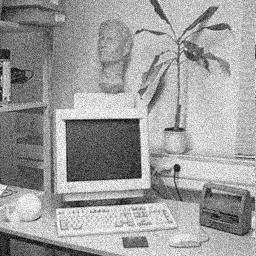
\includegraphics[scale=.5]{pics/office-noisy-1.jpg}}
\quad
\subfloat[]["Image 2"]{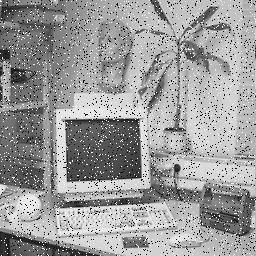
\includegraphics[scale=.5]{pics/office-noisy-2.jpg}}
\quad
\subfloat[]["Median filter Im 1 3x3"]{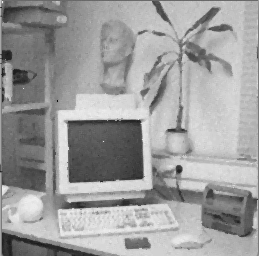
\includegraphics[scale=.5]{pics/2med_3.png}}
\quad
\subfloat[]["Median filter Im 2 3x3"]{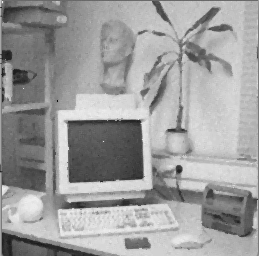
\includegraphics[scale=.5]{pics/2med_3.png}}
\quad
\subfloat[]["Median filter Im 1 9x9"]{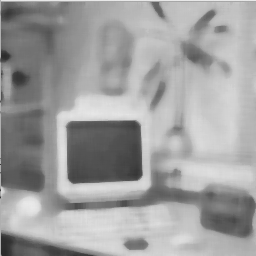
\includegraphics[scale=.5]{pics/1med_9.png}}
\quad
\subfloat[]["Median filter Im 2 9x9"]{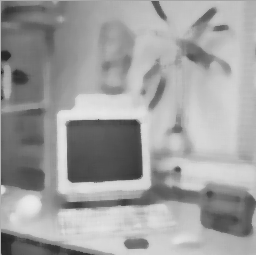
\includegraphics[scale=.5]{pics/2med_9.png}}
\quad

\caption{Comparison of different filter kernel size for median filter. The median filter with kernel size 3x3 works very well to reduce the noise in image 2, where the gaussian and the blur filter failed.}%
\label{fig:mblur}%
\end{figure}

\subsection{Filter Effects}
Both the blur filter and the gaussian work well to reduce noise in the image 1. I found that a 5x5 kernel size works very well to reduce the artificially introduced random noise. The gaussian filter seems to introduce less blurring of the features for equal kernel size compared to the blur filter (compare Fig.\ref{fig:blur}e and Fig.\ref{fig:gblur}e). Which makes sense, since neighbours closer to the center pixel are weighted stronger. Neither of the linear filter works well for Image two with "salt and pepper" noise. Although the specs are reduced, they are still clearly visible. 

This is expected, since these erroneous pixels are usually far away from their true value, which will pull the unweighted or weighted means as well. For random noise, the observed value is ususally close to the actual value, the mean based filters therefor work well.
These shortcomings are avoided by the median filter, since the median is in general less affected by outliers such as the ones produced by the salt and pepper noise.

All the filters make use of the fact that usually the intensity of a single pixel strongly correlates with the intensity of its neighbours.



\subsection{The Laplacian}
Edge detection is a very important and frequently encountered problem in image processing. Detecting edges in visual scenes seems to be a very trivial task for us. But what actually "makes" an edge? If we look at the pixel intensity of an image, edges are characterized by a very fast change of intensity over space. If we look at the one dimensional case and model pixel intensity by $I(x)$, finding edges corresponds to finding maximas in $\dot{I}(x)$ or finding $x$ such that $\ddot{I}(x) = 0$. In two dimensional images, this corresponds to applying the laplacian operator to the two dimensional intensity function and finding the zero crossings.:
\begin{equation}
\nabla I=\frac{\delta^{2} I}{\delta x^{2}} + \frac{\delta^{2} I}{\delta y^{2}}
\end{equation}

Fig. \ref{fig:lap} shows the laplacian of an image and the difference to the original.

\begin{figure}%
\centering
\subfloat[]["Original Image"]{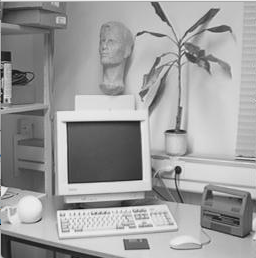
\includegraphics[scale=.35]{pics/office_orig.png}}
\quad
\subfloat[]["Laplace Transformation"]{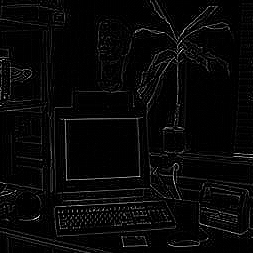
\includegraphics[scale=.35]{pics/office_lap.png}}
\quad
\subfloat[]["Difference"]{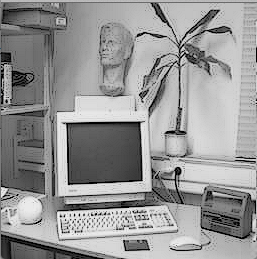
\includegraphics[scale=.35]{pics/office_dif.png}}

\caption{Laplace Operator. a) Original Picture. b) White pixels denote zero values of the laplacian. c) Difference between the original picture and the laplacian. Edges seem to be enhanced.}%
\label{fig:lap}%
\end{figure}


\end{document}